\documentclass[11pt,a4paper]{article}
\usepackage{wrapfig}
\usepackage{lastpage}
\usepackage[utf8]{inputenc}
\usepackage[pdftex,hyperfigures,hyperindex,bookmarksnumbered,colorlinks, bookmarks, breaklinks, linktocpage,citecolor=blue,urlcolor=blue,linkcolor=black,]{hyperref}
\usepackage{graphicx}
\usepackage{bm}
\usepackage{amsmath} 
\usepackage{amssymb}  
\usepackage{booktabs,multirow}

\usepackage{todonotes}
\usepackage{paralist}

\usepackage{physics}

\usepackage[binary-units=true]{siunitx}
\usepackage[caption=false]{subfig}

\graphicspath{{./figures/}} %Setting the graphicspath

%add subsubsubsection command
\makeatletter
\newcounter {subsubsubsection}[subsubsection]
\renewcommand\thesubsubsubsection{\thesubsubsection .\@arabic\c@subsubsubsection}
\newcommand\subsubsubsection{\@startsection{subsubsubsection}{4}{\z@}%
                                     {-3.25ex\@plus -1ex \@minus -.2ex}%
                                     {1.5ex \@plus .2ex}%
                                     {\normalfont\normalsize\bfseries}}
\newcommand*\l@subsubsubsection{\@dottedtocline{3}{10.0em}{4.1em}}
\newcommand*{\subsubsubsectionmark}[1]{}
\makeatother

\newcommand{\trsp}{{\scriptscriptstyle\top}}



\usepackage{geometry}
\geometry{a4paper, right=2cm, bottom=2.5cm, textwidth=17cm, textheight=24cm}
\usepackage{fancyhdr}
\pagestyle{fancy}

\usepackage[style=numeric, giveninits=true, defernumbers=true, backend=bibtex, maxnames=2, sorting=none, doi=false, isbn=false, url=false, eprint=false]{biblatex}
\usepackage{pdfpages} 
\title{Exploration of control strategies for a three-link 2D biped}
\author{Teguh Santoso Lembono}

\addbibresource{main.bib}



\begin{document}


\maketitle

\section{Introduction}
\label{sec:introduction}

The purpose of this report is to present a modelling, simulation, and control of a simplified humanoid robot walking model. The report is divided into two parts. The first presents the kinematics and dynamics analysis of the walking model, the impact map, the numerical integration for simulation, and the standard controller. The second part then presents the proposed controller using an optimal control approach. 






\section{Theory}
\label{sec:theory}

\begin{figure}[h!]
\centering
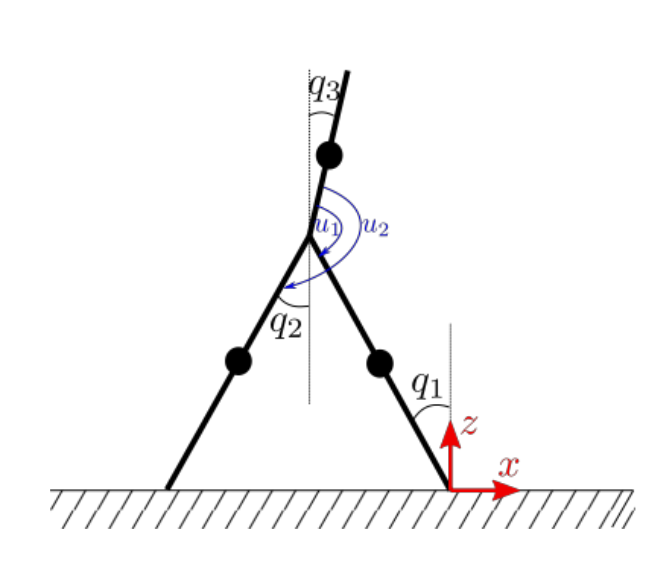
\includegraphics[width = 0.4\columnwidth]{simplified_model}
\caption{The simplified humanoid model used in this report.}
\label{fig:simplified_model}
\end{figure}

The simplified model of the humanoid is shown in Fig.~\ref{fig:simplified_model}. It is represented by three-links model, two refer to the legs and one for the torso. Each link has a point mass at its center. At each instant, one leg acts as the stance leg that stays stationary, and the other as the swing leg. 

\subsection{Kinematics}
\label{sec:kine}
The kinematics can be easily calculated by considering the stance foot location as the origin of the coordinate frame, as shown in Fig.~\ref{fig:simplified_model}. The points of interests are then the location of each mass ($\bm{r}_1, \bm{r}_2, \bm{r}_3$), the torso ($\bm{r}_t$), the hip ($\bm{r}_h$), and the swing foot ($\bm{r}_{swf}$). Each point $\bm{r}$ consists of the $x$ and $z$ coordinates. By simple geometry, we obtain
\begin{align}
x_1 = &  0.5*l_1*sin(q_1) \\
z_1 = & 0.5*l_1*cos(q_1) \\
x_2 = & l_1*sin(q_1)-0.5*l_2*sin(q_2) \\
z_2 = & l_1*cos(q_1)-0.5*l_2*cos(q_2) \\
x_3 = & l_1*sin(q_1)+ 0.5*l_3*sin(q_3) \\
z_3 = & l_1*cos(q_1)+ 0.5*l_3*cos(q_3) \\
x_h = & l_1*sin(q_1) \\
z_h = & l_1*cos(q_1) \\
x_{swf} = & l_1*sin(q_1)-l_2*sin(q_2) \\
z_{swf} = & l_1*cos(q_1)-l_2*cos(q_2) \\
x_t = & l_1*sin(q_1)+ l_3*sin(q_3) \\
z_t = & l_1*cos(q_1)+ l_3*cos(q_3).
\end{align}

The corresponding velocities can then be computed using chain rule, i.e.
\begin{equation}
\dv{\bm{r}}{t} = \pdv{\bm{r}}{\bm{q}} \pdv{\bm{q}}{t}.
\end{equation}

Using the symbolic programming in matlab or python, the velocity calculation can be done automatically. 

\subsection{Dynamics}
\label{sec:dyn}
To obtain the dynamic equation of the locomotion model, the dynamics is divided into two phases: the swing phase and the impact phase. In the swing phase, we assume that the stance foot is not moving (there is sufficient contact force to keep it stationary), while the swing foot is moving to the next contact location. At the point of impact, we assume an instantaneous impact that preserves the momentum, as described in the next section. 

To describe the dynamics of the swing phase, we can rely on Lagrangian dynamics. First, we found the expression of the total kinetic and potential energy ($T$ and $V$),
\begin{align}
T = & \sum_{i=1}^{3} \frac{1}{2} m_i \dv{\bm{r}_i}{t}^2 \\
V = & \sum_{i=1}^{3} m_i g z_i.
\end{align}

The Lagrangian is then calculated as 
\begin{equation}
L = T - V . 
\end{equation}

With this, the Lagrangian equation of motion can be calculated as
\begin{equation}
\frac{d}{dt} (\pdv{L}{\dot{q}_i}) - \pdv{L}{q_i} = \tau_i,
\label{eq:total_lagrange}
\end{equation}
where $\tau_i$ is the generalized torque. The equations can be computed using the symbolic programming. 

After obtaining the equations for $i = 1, 2, 3$, we can rearrange them in the following form, 
\begin{equation}
\bm{M}(\bm{q})\ddot{\bm{q}} + \bm{C}({\bm{q}},\dot{\bm{q}})\dot{\bm{q}} + \bm{G}({\bm{q}}) = \bm{\tau}. 
\label{eq:total_standard}
\end{equation}

The terms $\bm{M}(\bm{q}), \bm{C}({\bm{q}},\dot{\bm{q}})$, and $\bm{G}({\bm{q}})$ can be computed from \eqref{eq:total_standard} as follows. $\bm{G}(\bm{q})$ is computed by setting $(\dot{\bm{q}}, \ddot{\bm{q}}, \bm{\tau})$ in \eqref{eq:total_standard} to zero. 
$\bm{M}(\bm{q})$ is computed by setting $(\dot{\bm{q}},\bm{\tau})$ in \eqref{eq:total_standard} to zero, substracting the term $\bm{G}(\bm{q})$ from the equation. Finally, $\bm{C}(\bm{q}, \dot{\bm{q}})$ is computed by setting 
$(\ddot{\bm{q}}, \bm{\tau})$ to zero, substracting the term $\bm{G}(\bm{q})$ from the equation, and dividing by the corresponding $\dot{\bm{q}}$. 

\subsection{Impact Map}
\label{sec:impact}

\begin{figure}[h!]
\centering
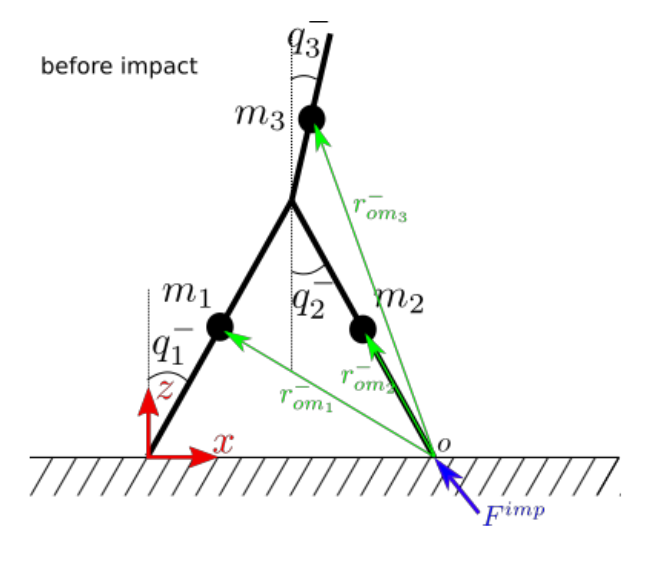
\includegraphics[width = 0.4\columnwidth]{before_impact}
\hspace{0.5cm}
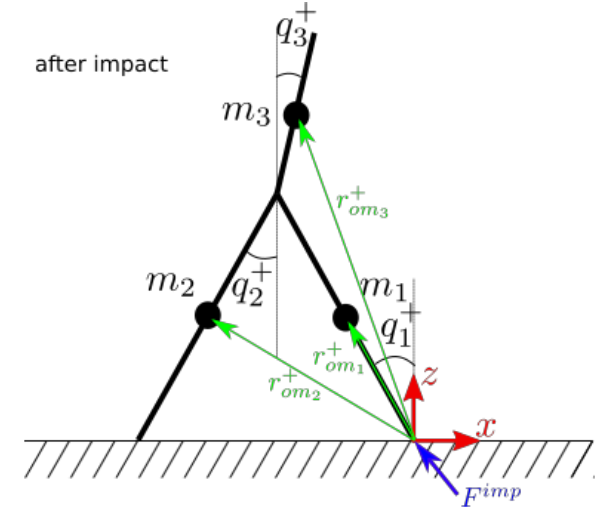
\includegraphics[width = 0.4\columnwidth]{after_impact}
\caption{Diagram for angular momentum conservation at the impact point. \emph{Left}: before impact, \emph{right}: after impact. }
\label{fig:impact}
\end{figure}


\begin{figure}[h!]
\centering
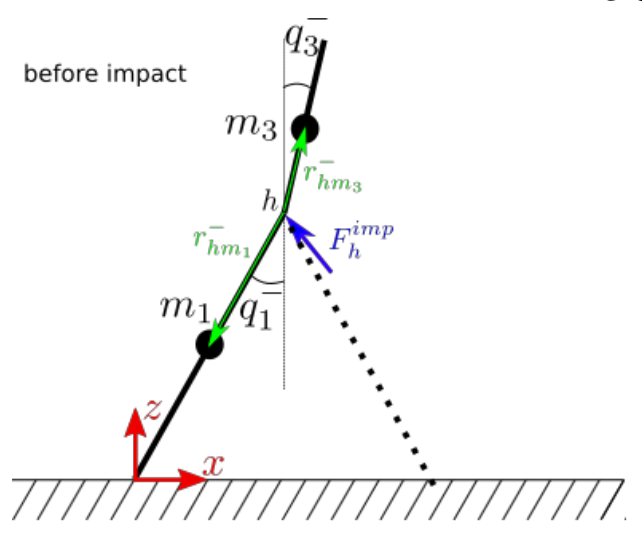
\includegraphics[width = 0.4\columnwidth]{before_impact2}
\hspace{0.5cm}
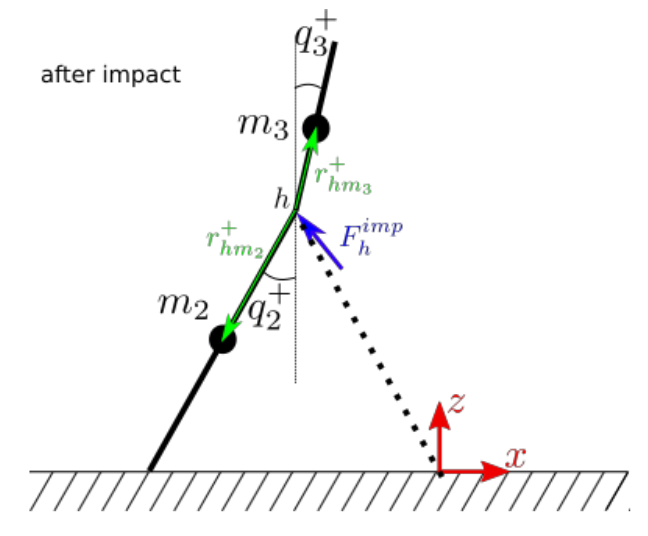
\includegraphics[width = 0.4\columnwidth]{after_impact2}
\caption{Diagram for angular momentum conservation at the hip. \emph{Left}: before impact, \emph{right}: after impact. }
\label{fig:impact2}
\end{figure}


In our model, after the impact we switch the swing foot to become the stance foot, as shown in Fig.~\ref{fig:impact} (left: before impact, right: after impact). The angles are therefore changed as follows,
\begin{align}
q_1^+ = & q_2^- \\
q_2^+ = & q_1^- \\
q_3^+ = & q_3^-,
\end{align}
the superscripts $(^-, ^+)$ refer to the variables before and after impact, respectively. 

The impact map for the angular velocity can be computed by considering the conservation of angular momentum at the impact at two locations: the impact point (the location of the swing foot at the impact), and at the hip. 

Looking at Fig.~\ref{fig:impact} and \ref{fig:impact2}, the momentum before the impact can be written as:
\begin{alignat}{2}
H_a^- = & \quad\sum_{i=1}^{3} m_i \bm{r}_{{om}_i}^{-} \cross \dot{\bm{r}_i}^{-} && = \quad \sum_{i=1}^{3} m_i (\bm{r}_i^{-} - \bm{r}_{swf}^{-}) \cross \dot{\bm{r}_i}^{-}\\
H_b^- = &\quad m_1 \bm{r}_{hm_1}^- \cross \dot{\bm{r}_1^-} && = \quad m_1 (\bm{r}_{1}^- - \bm{r}_{h}^-) \cross \dot{\bm{r}_1^-} \\
H_c^- = &\quad m_3 \bm{r}_{hm_3}^- \cross \dot{\bm{r}_3^-} && = \quad m_3 (\bm{r}_3^- - \bm{r}_h^-) \cross \dot{\bm{r}_3^-},
\end{alignat}
and after impact as
\begin{alignat}{2}
H_a^+ = &\quad \sum_{i=1}^{3} m_i \bm{r}_{{om}_i}^{+} \cross \dot{\bm{r}_i}^{+} && = \sum_{i=1}^{3} m_i \bm{r}_i^{+} \cross \dot{\bm{r}_i}^{+}\\ 
H_b^+ = & \quad m_1 \bm{r}_{{hm}_2}^+ \cross \dot{\bm{r}_2^+} && = m_1 (\bm{r}_{2}^+ - \bm{r}_{h}^+ ) \cross \dot{\bm{r}_2^+} \\
H_c^+ = & \quad m_3 \bm{r}_{{hm}_3}^+ \cross \dot{\bm{r}_3^+} && = m_3 (\bm{r}_{3}^+ - \bm{r}_{h}^+) \cross \dot{\bm{r}_3^+}.
\end{alignat}

We can rearrange the equations to obtain $\bm{H}^- = \bm{A}_{\_} \dot{\bm{q}}^-$ and $\bm{H}^- = \bm{A}_{+} \dot{\bm{q}}^+$. Then we can obtain the velocities after the impact by solving the linear equation $\bm{H}^- = \bm{H}^+$, 
\begin{equation}
\dot{\bm{q}}^+ = \bm{A}_{+}^{-1} \bm{A}_{\_}  \dot{\bm{q}}^-. 
\end{equation}

\subsubsection{Exercise Answers}
\begin{itemize}
\item Q: \emph{What can you say about the potential energy before and after impact?} 
The potential energy before and after impact do not differ, because the position of each mass remains the same. What changes after the impact is only the kinetic energy.
\item Q: \emph{Try $q_m = [\pi/6, -\pi/6, \pi/10], dq_m = a[1, 0.2, 0]$. What percentage of the kinetic energy of the biped is lost due to the impact?}  
There is 27.92\% of the kinetic energy lost due to the impact. 
\item Q: \emph{Plot the percentage of the kinetic energy loss due to impact as a function of angle $\alpha$ where $q^- = [\alpha, -\alpha, 0]$  and $\alpha$ varies from 0 to $\pi/4$. Assume that $\dot q^- = [1, 0.2, 0]$. Include your plot.}
\centering{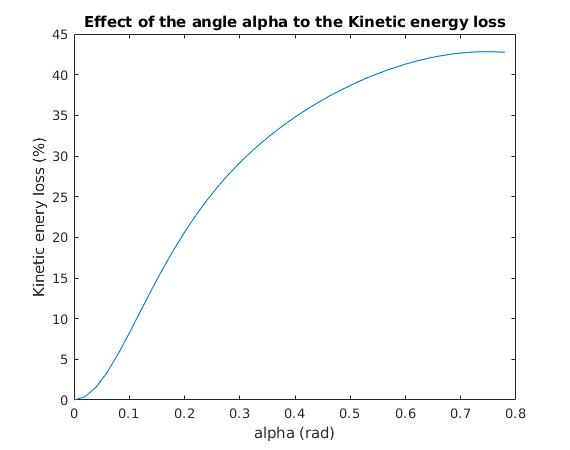
\includegraphics[width=0.6\columnwidth]{alpha_kineticloss}}

\raggedright \item Q: \emph{The bigger $\alpha$ is the bigger is the step length. Based on your answer to question 3, what is the relation between step length and energy loss at impact given a fixed $\dot q^-$?}
As the step length grows bigger, the energy loss increases.    
\end{itemize}

\subsection{Model Validation and Animation}
\label{sec:validation}
Using the kinematics, dynamics, and impact map functions, we can run a simulation of the locomotion model, given a particular controller. The simulation is run using numerical integration, which is described in the next section. 
%
\subsubsection{Exercise Answers}
\begin{itemize}
\item \emph{ In the animations, what does a real-time factor of 1 mean? How about a real-time factor less than 1?}
The real time factor describes the ratio between the actual time taken by the motion and the animation time. Real time factor of 1 means that the duration of the animation that appears to us is exactly the same as the duration of the actual step according to the model. Real time factor less than 1 means that the animation appears slower than the actual motion.
\item \emph{How does “skip” in animate.m effect the real-time factor and the speed of the animation?}
The variable "skip" determines how many data points that we do not show in the animation. The larger this value is, the sparser the animation is, and the faster it is. Hence, as "skip" increases, the real time factor will increase and the animation speed becomes faster.
\item \emph{What is the role of r0 in animate.m?}
r0 is the location of the supporting foot. This is necessary because the coordinates of the other points are described with respect to this point. As the supporting foot changes at the impact, the value of r0 is updated correspondingly. 
\end{itemize}

\subsection{Numerical Integration}
\label{sec:num_int}

At each step, we run the numerical integration of the swing phase dynamics, while checking if the swing foot crosses the ground. This can be defined as an event function that is checked in the numerical integrator at each function evaluation. For the integrator, I am using \emph{solve\_ivp} from the scipy library in python. 

\subsubsection{Exercise Answer for Explicit Euler}
\begin{figure}[h!]
\centering
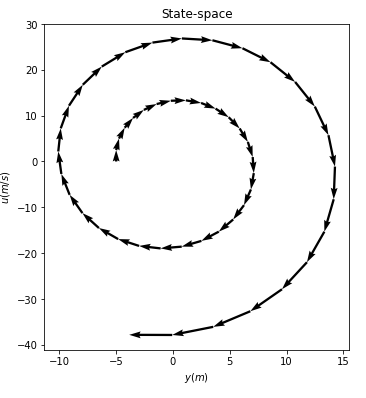
\includegraphics[width=.4\columnwidth]{exp_euler1}
\quad
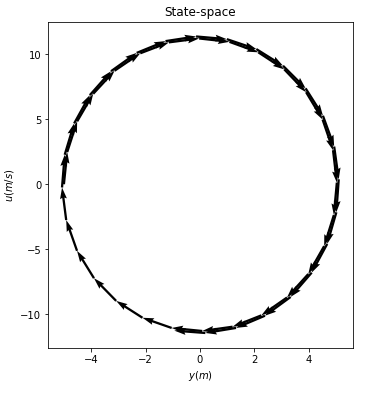
\includegraphics[width=.4\columnwidth]{exp_euler2}
\caption{State space plot for explicit euler. \emph{Left}: $dt =0.1$, \emph{right}: $dt = 0.002$.}
\label{fig:exp_euler}
\end{figure}


\begin{itemize}
\item \emph{Explain the meaning of the state-space plot (right subfigure). What should be the expected state-space plot (hint: change visualize function)?}
The state space plot shows the evolution of the joint angle $\bm{q}$ and its velocity $\dot{\bm{q}}$ over time. Since the damping coefficient here is zero, the system should have a stable oscillation, i.e. the movement should be periodical and after one period we should go back to the same point on the phase plot. What is shown here, though, is a spiralling movement whose radius is increasing, showing that the energy of the system increases as time goes on, due to the inaccuracy of Explicit Euler method.
\item \emph{Why does the numerical solution diverges from the true solution (hint: Taylor expansion)?}
Explicit Euler uses a first order Taylor expansion to approximate the integration, this results in a quite significant error, especially when the time interval is large (0.1 in this case). This results in energy increase as the integration is performed, resulting in the divergence.
\item \emph{What can you do to better approximate the actual solution with this method?}
We can decrease the time interval to reduce the error. Fig.~\ref{fig:exp_euler} (right) shows the phase plot for dt = 0.002, which has an almost circular shape (stable limit cycle).
\end{itemize}

\subsubsection{Exercise Answer for Semi-implicit Euler}
\begin{itemize}

\item \emph{Is this method stable and when?}
By looking at the phase plot, the method seems to be quite stable, although the shape does not fit a perfect circle (meaning a non-negligible error, although the error is not accumulating). 

\item \emph{What about the accuracy of the obtained solution?}
The accuracy can be computed as the mean squared error $e = \frac{1}{N} \sum_{n=1}{N} (\bm{y}-\bm{y}_{\text{true}})^2$. For $dt = 0.1$, the error is $e = 0.202$.  
\end{itemize}

\subsubsection{Exercise Answer for Runge-Kutta}
\begin{itemize}
\item \emph{What is the error of this method?}
The mean squared error is $e = 2.58e-7$ for $dt = 0.1$, which is much lower than Semi-implicit euler method. 

\item \emph{Do you expect the solution to diverge?}
Looking at the phase plot, it does not seem to diverge. The error is also very small. 
\end{itemize}

\subsubsection{Exercise Answer for Adaptive Time Stepping}
\begin{itemize}

\item \emph{Change the density of the time points in np.linspace. What do you observe?}
With different density, the solution seems to remain quite stable. Even with very low density, the solution is still stable. 
\item \emph{Do you expect the solution to diverge?}
Looking at the phase plot, it seems to make a stable limit cycle and does not seem to diverge.
\item \emph{Which algorithms are supported by odeint?}
Odeint supports 'LSODA' from FORTRAN library. The newer algorithm for numerical integration seems to be \emph{solve\_ivp}, which supports 'RK45', 'RK23', 'DOP853', 'Radau', 'BDF', and 'LSODA'. 
\end{itemize}

\subsection{Control and Optimization}
\label{sec:control_opt}

The system during the swing phase is underactuated, i.e. there are three degrees of freedom to control but only two control inputs, as shown in Fig.~\ref{fig:control}. In the standard controller, we first choose the first control input $u_1$ to control the torso angle to be at a desired value $\alpha$, whereas the second control input $u_2$ is used to control the swing foot angle $q_2$. Expressing these as virtual constraints in terms of new variables $y_1$ and $y_2$, we set
\begin{align}
y_1 = q_3 - \alpha \\
y_2 = -q_2 - q_1. 
\end{align}

Differentiating this constraint, we obtain
\begin{align}
\dot{y}_1 = \dot{q}_3  \\
\dot{y}_2 = -\dot{q}_2 - \dot{q}_1. 
\end{align}

We then set the controller as PD control to drive $y_1, y_2$ to zeros,
\begin{align}
u_1 = k_1^P y_1 + k_1^D \dot{y}_1 \\
u_2 = k_2^P y_2 + k_2^D \dot{y}_2.
\end{align}

Now what is left is to choose the parameters $(k_1^P, k_1^D, k_2^P, k_2^D, \text{and} \alpha)$, as well as the initial state $(\bm{q}^0, \dot{\bm{q}}^0)$. We use the function $\emph{fmin}$ in Matlab to optimize these parameters, given an objective function. 

\subsubsection{Objective function for optimizing the standard controller}
For this part, I use the standard objective function given in the exercise,
\begin{equation}
F(\bm{\Phi}) = w_1*|\epsilon - \epsilon_d| + w_2*CoT,
\end{equation}
where $w_1$ and $w_2$ are the weights and $CoT$ is the cost of transport (as defined in the exercise). $\epsilon$ refers to the criteria of interest (e.g. velocity, step length, frequency), and $\epsilon_d$ is the desired value. Since CoT typically has high value, $w_2$ is set to be quite small, typically 3 order lower than $w_1$ (e.g. $w_1 = 3, w_2 = 1000$). The CoT term is useful to help the motion to be stable, even when we do not want to minimize CoT. 

\subsubsection{Result}



\renewcommand{\arraystretch}{1.}
\begin{table}[!t]
	\centering    
      \caption{Parameters for standard controller}
      \label{tab:standard_result}
		
	\begin{tabular}{l l | c  c  c }
		\toprule
\bf{Criteria} & \bf{Value} & $\bm{q}_0$ & $\dot{\bm{q}_0}$ & $(k_1^P, k_2^P, k_1^D, k_2^D, \alpha)$ \\
\bf{Velocity} & 0.2 & (-0.283856, 0.345331, 0.005407) & ( 0.758883, -0.323396, 2.114896) & (476.490262, 160.040142, 72.798758, 7.454037, 0.001594) \\
\bf{Velocity} & 0.9 & (-0.3711,   0.3816,   0.1293) & (  0.6068,  -1.1616,   3.8571) & ( 352.0519, 179.2402,  80.1826,   4.6536,   0.1947) \\
\bf{Frequency} & 0.7 & (-0.283856, 0.345331, 0.005407) & ( 0.758883, -0.323396, 2.114896) & ( 476.490262, 160.040142, 72.798758, 7.454037, 0.001594 )\\
\bf{Frequency} & 3.7 & (-0.168262, 0.260154, -0.014194) & ( 1.858029, 1.356398, 0.034423) & ( 304.269003, 189.627411, 134.508350, -0.045500, -0.183163) \\
\bf{Step Length} & 0.21 & (-0.168262, 0.260154, -0.014194) & ( 1.858029, 1.356398, 0.034423) & ( 304.269003, 189.627411, 134.508350, -0.045500, -0.183163) \\
\bf{Step Length} & 0.4 & (-0.037315, -0.610571, 0.000515) & ( 0.000042, 0.156022, 5.790911) & ( 244.527802, 269.296473, 53.476705, 6.514429, 0.156793) 
	\end{tabular}
\end{table}
\section{Control}
\label{sec:control}


\subsection{Overview of Control Strategy}
\label{sec:overview}

In this work, I rely on \emph{optimal control} to design an efficient locomotion controller. The advantage of this formulation is that the resulting motion is optimal w.r.t. the desired criteria, which can be expressed as an objective function and constraint(s). A high level specification (such as minimizing energy, tracking a desired foot trajectory, tracking a desired torso angle) can be translated quite easily to the objective function. 

However, there are several challenges in implementing the optimal controller to this problem. Firstly, most optimal control strategy in robotics is time-based. That is, given a time horizon (e.g. 1 second), solving the optimal control problem will give us a specific control and state trajectory that minimizes the objective function while satisfying the constraints. Some variants are time independent, e.g. when the time horizon is infinite, but it is not suitable for this locomotion problem (where the desired behavior highly depends on time and event, and not stationary). Since the impact timing is difficult to predict precisely (especially given some disturbance), a purely time-based controller is difficult to be used here. Secondly, the dynamics model of our locomotion is discontinuous due to the impact map. This is a big problem for optimal control, as most methods would require the gradient of the dynamics function. 

To overcome these issues, I propose to use the following approach. First, the optimal control is solved for only one step until impact, so that the discontinous event at the impact is not considered. Considering that the locomotion is a periodical motion, designing an optimal trajectory for one step should be sufficient, provided that the state after the impact returns to the initial state. 
Secondly, we need a controller that is not purely time based or feed forward only. One option is to use a feedback controller (e.g. PD) to track the desired optimal trajectory. However, there is a specific optimal control formulation that provides this automatically, i.e. Iterative Linear Quadratic Regulator (ILQR). Solving ILQR gives us both the optimal trajectories and the optimal feedback controller (note that 'optimal' here refers to local optimum, not the global one). 
Finally, to choose the optimum parameters for the optimal control, we again rely on an optimization solver (fmin) to ensure that the controller is stable.

\subsection{Iterative Linear Quadratic Regulator (ILQR)}
\label{sec:ilqr}

A general discrete OCP consists of a cost function
\begin{equation}
C(\bm{x}, \bm{u}) = \sum_{t=0}^{T-1} c_t(\bm{x}_t, \bm{u}_t) + c_T(\bm{x}_T, \bm{u}_T),
\label{eq:general_cost}
\end{equation}
subject to the dynamics
\begin{equation}
\bm{x}_{t+1} = \bm{f}(\bm{x}_t, \bm{u}_t).
\label{eq:general_dynamics}
\end{equation}
$(\bm{x}, \bm{u})$ are the state and control trajectories for the time horizon $T$. ILQR solves this optimal control problem by iteratively formulating a sub problem as an LQR problem and solve it to obtain a better solution at each iteration.

Let us consider the current guess $(\bm{x}^k, \bm{u}^k)$, where $k$ is the iteration index. Given the general cost function in \eqref{eq:general_cost}, we approximate it as a quadratic function around $(\bm{x}^k, \bm{u}^k)$,
\begin{multline} 
\hfill
\centering
c_t(\delta\bm{x}_t, \delta\bm{u}_t) = \frac{1}{2} 
\begin{bmatrix}
\delta \bm{x}_t \\ \delta \bm{u}_t 
\end{bmatrix}
^\trsp
\begin{bmatrix}
\bm{c}_{\bm{xx},t} & \bm{0} \\ \bm{0} & \bm{c}_{\bm{uu},t}
\end{bmatrix}
\begin{bmatrix}
\delta \bm{x}_t \\ \delta \bm{u}_t 
\end{bmatrix}
 + 
\begin{bmatrix}
\bm{c}_{\bm{x},t} &  \bm{c}_{\bm{u},t}
\end{bmatrix}
\begin{bmatrix}
\delta \bm{x}_t \\ \delta \bm{u}_t 
\end{bmatrix},
\label{eq:quadratized_cost}
\end{multline}
where $\bm{c}_{\bm{x},t}, \bm{c}_{\bm{u},t}, \bm{c}_{\bm{xx},t},$ and $\bm{c}_{\bm{uu},t}$ are the cost function's first and second order derivatives with respect to $\bm{x}$ and $\bm{u}$. Similarly, we can approximate the dynamics in \eqref{eq:general_dynamics} using the linear approximation
\begin{equation}
\delta \bm{x}_t = \bm{A}_t \delta \bm{x}_t + \bm{B}_t \delta \bm{u}_t,
\label{eq:linearized_dynamics}
\end{equation}
where $\bm{A}_t$ and $\bm{B}_t$ are the derivatives of the dynamics $\bm{f}(\bm{x}_t, \bm{u}_t)$ with respect to $\bm{x}_t$ and $\bm{u}_t$, respectively. The derivatives are evaluated at the current guess $(\bm{x}^k, \bm{u}^k)$. At this stage, we have quadratic costs and linear dynamics as functions of $\delta\bm{x}$ and $\delta\bm{u}$. This is therefore a time-varying LQR problem, of which the variables of interest are $\delta\bm{x}$ and $\delta\bm{u}$, and the solution can be computed analytically. 

By the end of ILQR iteration, we will have a locally optimal solution as state and control trajectories $(\bm{x}^*, \bm{u}^*)$, as well as the optimal feedback term $\bm{K}_t$. To use this feedback term, at online execution we compute the control command by 
\begin{equation}
\bm{u}_t = \bm{u}_t^* + \bm{K}_t (\bm{x}_t - \bm{x}_t^*).
\end{equation}
This optimal feedback term serves as a locally optimal PD controler to track the optimal trajectories $(\bm{x}^*, \bm{u}^*)$. 

\subsection{ILQR formulation for the locomotion}
For the locomotion problem, we consider the initial state $\bm{x}_0$ to be the state right after an impact, and the end state $\bm{x}_T$ to be at the next predicted impact. It turns out that formulating the objective function for this problem is complicated, due to the event detection. I previously try using an objective function to only reach the desired end state $\bm{x}_T$, but this often results in failure because the swing foot touches the ground before reaching $\bm{x}_T$. In this event based detection, the swing foot trajectory is very important. Another variable that is also important is the torso angle ($\bm{q}_3$). This needs to be kept small enough, otherwise the motion is often unstable. 

After a lot of trials, the objective function that is found to be working is to track a desired foot swing trajectory, while keeping the torso angle to be around a desired angle. The running cost, i.e. the cost for $t = [0, T-1] $ is set to be
\begin{equation}
c(\bm{x}_t, \bm{u}_t) = (\bm{r}_{swf, t} - \bm{r}_{swf, t}^*)^\trsp \bm{W} (\bm{r}_{swf,t} - \bm{r}_{swf, t}^*) + \lambda (q_{3,t} - \alpha)^2 +  \bm{u_t}^T \bm{R} \bm{u}_t,
\end{equation}
while the terminal cost at $t = T$ is set to be 
\begin{equation}
c(\bm{x}_T, \bm{u}_T) = (\bm{r}_{swf, T} - \bm{r}_{swf, T}^*)^\trsp \bm{W}_T (\bm{r}_{swf, T} - \bm{r}_{swf, T}^*) + \lambda (q_{3,T} - \alpha)^2.
\end{equation}

The constraint on the control input is a box constraint, 
\begin{equation}
-30 \leq \bm{u}_i \leq 30 \quad \text{for} \quad  i = 1, 2 . 
\end{equation}

To solve this constrained ILQR problem, I use the open source solver Crocoddyl. It uses the box-FDDP algorithm that accepts infeasible initial guess $(\bm{x}^0, \bm{u}^0)$. 

\subsection{Optimization Strategy}
\label{sec:opt_strat}

To use the optimal control formulation, we have to choose the following parameters $\bm{\Phi}$:
\begin{itemize}
\item The initial state $(\bm{q}_0, \dot{\bm{q}_0})$
\item The desired torso angle $\alpha$
\item The desired goal position for the swing foot $x_{swf,T}^*$
\end{itemize}

Although optimal control formulation is powerful, finding the optimal parameters for a desired objective of this particular locomotion problem turns out to be challenging. Instead of starting from random initial guess, I rely on the standard controller discussed in Section~\ref{sec:control_opt}. For a given desired criteria (e.g. a desired speed, step length etc.), first I optimize this standard controller to achieve the criteria, and observe the corresponding parameters $\bm{\Phi}$ as well as the time interval $T$. Using this with the ILQR often results in failure, i.e. unstable controller, as the ILQR is still time based and depend a lot on the impact event. So we need to further optimize $\bm{\Phi}$ to obtain a good controller.

To make the optimization tractable, I do it step by step. First, I optimize for only one foot step. Since a stable controller will have a stable limit cycle, the next state after the impact should be very close to the initial state. So I design the objective function for the optimization to be 
\begin{equation}
f(\bm{\Phi}) = ||\bm{x}_0 - \bm{x}_T^+ ||_2,
\end{equation}
where $\bm{x}_0$ is the initial state, and $\bm{x}_T^+$ is the final state after the impact (i.e. the initial state for the next foot step). By ensuring that $\bm{x}_0$ is as close as possible to $\bm{x}_T^+$, we can have a stable limit cycle. 

In practice, optimizing for only one foot step only makes a stable controller for a few foot steps, as the error diverges. When this happens, the optimization is run again, but this time with a longer foot steps, and initialized using the previously obtained parameters. Doing this iteratively often results in a controller that is stable for a large number of foot steps, even to infinity. 

\subsection{Results and Discussion}
\label{sec:results}

\renewcommand{\arraystretch}{1.}
\begin{table}[!t]
	\centering    
      \caption{Parameters for ILQR controller}
      \label{tab:ilqr_result}
		
	\begin{tabular}{l l | c  c  c c c c}
		\toprule
\bf{Criteria} & \bf{Value} & $\bm{q}_0$ & $\dot{\bm{q}_0}$ & $\alpha$ &  \bf{Step} & $T$ & $\lambda_{\phi}$\\
\bf{Vel} & 0.31 & (-0.17,  0.27,  0.05) & (  1.8 ,  0.99,  0.02) &   0.05 & 0.25 & 0.268 \\
\bf{Vel} & 0.877 &( -0.34,  0.39,  0.35) & (  0.78, -1.45,  5.44) &   0.34&       0.36 & 0.421\\
\bf{Freq} & 2.2 & (-0.34,  0.39,  0.35) & ( 0.79, -1.45,  5.44) &   0.34&0.36 &0.421  \\
\bf{Freq} & 3.65 & (-0.17 ,  0.27 ,  0.05) & (  1.84,  0.99,  0.02) &   0.05 &        0.25 &0.268 \\
\bf{Step} & 0.117 &(-0.17,  0.27,  0.05) & (  1.84 ,  0.99,  0.02) &  0.05& 0.25& 0.268\\
\bf{Step} & 0.372 &(-0.34,  0.39,  0.35) & (  0.79, -1.45,  5.44) &   0.34& 0.36& 0.421 
	\end{tabular}
\end{table}




\begin{figure}
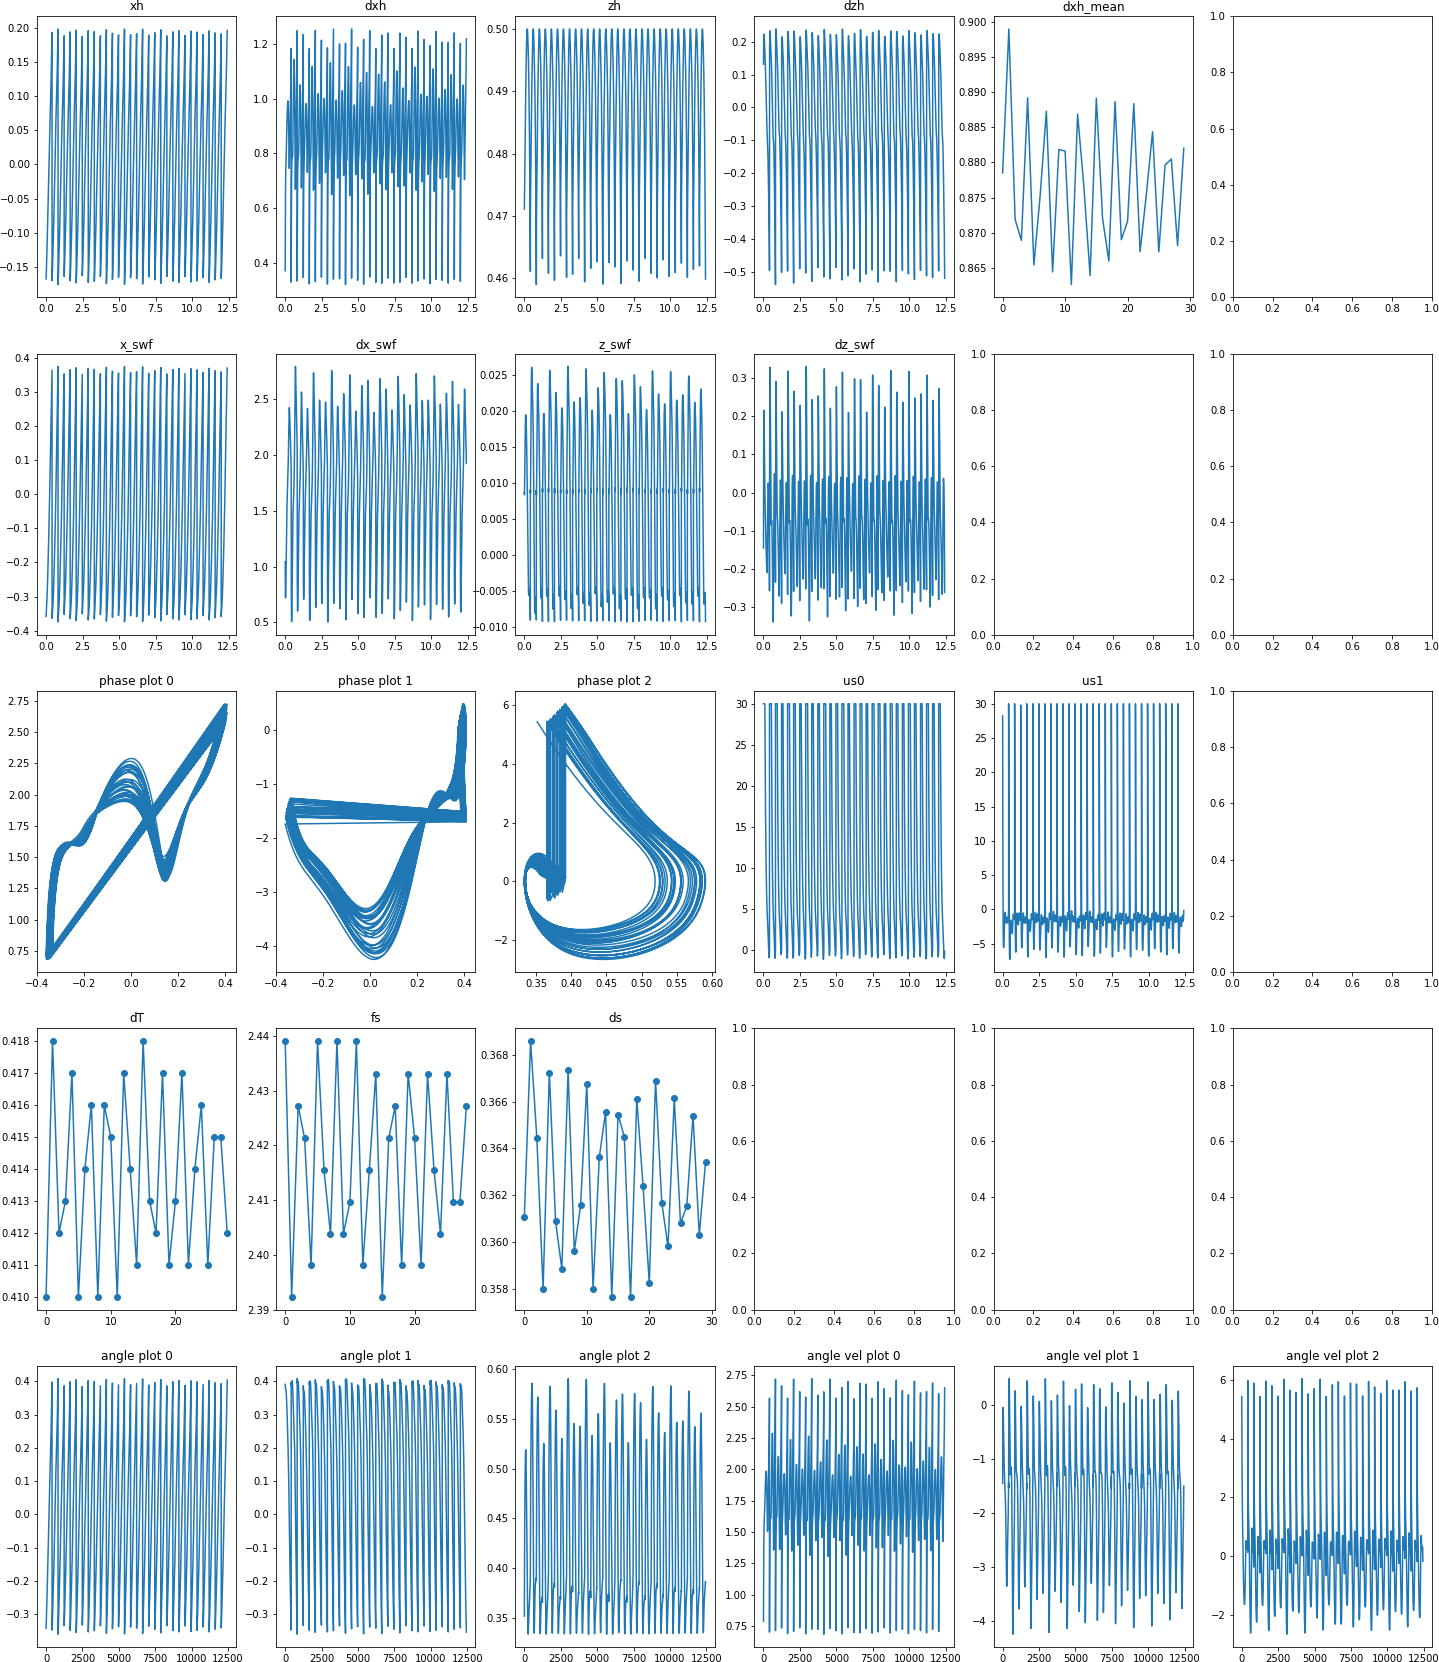
\includegraphics[width=0.99\columnwidth]{example_v09_prev}
\caption{Various plots for the ILQR controller simulation with velocity = 0.877}
\label{fig:ilqr_plot}
\end{figure}

\subsection{Conclusion}
\label{sec:conclusion}

\section{Conclusion}
\label{sec:conclusion}

In this report, I have presented an optimal control formulation for a simplified 2D humanoid robot walking model. The parameters are optimized for various criteria (speed, step length, frequency), and robustness towards perturbation has been characterized. The optimal control problem is solved using ILQR, which is quite popular in robotics due to its fast computation. In addition, ILQR provides us not only with the optimal state and control trajectory, but also the feedback controller. From the simulation, we observe that ILQR can result in 30-40\% lower Cost of Transport than the standard controller.

However, the formulation poses several difficulties. Firstly, choosing the objective function is not too easy. I set the objective function to mainly track the desired foot trajectory while keeping the torso at a specified angle. Secondly, the impact map results in discontinuity of the dynamics, which is a big problem for optimal control in general. I solve this by computing the optimal control for one foot step, and optimize the parameters such that the motion reaches a stable limit cycle. 

While the resulting controller performs well, it can be made even more stable by considering several possible approaches. If the computation time can be made faster, we can recompute the ILQR at each iteration, i.e. doing Model Predictive Control (MPC). We can also not use the feedback gain of ILQR and instead use another tracking controller, such as QP-based controller, or a shorter horizon MPC controller that can be computed faster, to track the optimal trajectory from ILQR. 








\newpage
%\bibliographystyle{IEEEtran} 
%\bibliography{references}
\printbibliography


\end{document}
